\documentclass[10pt,letterpaper]{report}
\usepackage[latin1]{inputenc}
\usepackage{amsmath}
\usepackage{amsfonts}
\usepackage{amssymb}
\usepackage{graphicx}
\usepackage{blindtext}
\usepackage{listings}
\usepackage{enumerate}
\usepackage{enumitem}
\usepackage{hyperref}
\usepackage{cancel}
\usepackage{color,soul}
\usepackage{multirow}
\usepackage{float}
\usepackage[left=1.00in, right=1.00in, top=1.00in, bottom=1.00in]{geometry}
\author{Derek Lontine, Stuart Childs, Alex Bailey}
\title{AFEM: Axisymmetric Project Verification Tests}

\usepackage{color}
 
\definecolor{codegreen}{rgb}{0,0.6,0}
\definecolor{codegray}{rgb}{0.5,0.5,0.5}
\definecolor{codepurple}{rgb}{0.58,0,0.82}
\definecolor{backcolour}{rgb}{0.95,0.95,0.92}
 
\lstdefinestyle{mystyle}{
    backgroundcolor=\color{backcolour},   
    commentstyle=\color{codegreen},
    keywordstyle=\color{magenta},
    numberstyle=\tiny\color{codegray},
    stringstyle=\color{codepurple},
    basicstyle=\footnotesize,
    breakatwhitespace=false,         
    breaklines=true,                 
    captionpos=b,                    
    keepspaces=true,                 
    numbers=left,                    
    numbersep=5pt,                  
    showspaces=false,                
    showstringspaces=false,
    showtabs=false,                  
    tabsize=2
}
\lstset{style=mystyle}

%Tensor notation undertildes
\usepackage{stackengine} 
\stackMath 
\newcommand\tenq[2][1]{ \def\useanchorwidth{T} \ifnum#1>1 \stackunder[0pt]{\tenq[\numexpr#1-1\relax]{#2}}{\scriptscriptstyle\sim} \else \stackunder[1pt]{#2}{\scriptscriptstyle\sim} \fi } 



\numberwithin{equation}{chapter}


\usepackage{empheq}
 
% Command "alignedbox{}{}" for a box within an align environment
% Source: http://www.latex-community.org/forum/viewtopic.php?f=46&t=8144
\newlength\dlf  % Define a new measure, dlf
\newcommand\alignedbox[2]{
% Argument #1 = before & if there were no box (lhs)
% Argument #2 = after & if there were no box (rhs)
&  % Alignment sign of the line
{
\settowidth\dlf{$\displaystyle #1$}  
    % The width of \dlf is the width of the lhs, with a displaystyle font
\addtolength\dlf{\fboxsep+\fboxrule}  
    % Add to it the distance to the box, and the width of the line of the box
\hspace{-\dlf}  
    % Move everything dlf units to the left, so that & #1 #2 is aligned under #1 & #2
\boxed{#1 #2}
    % Put a box around lhs and rhs
}
}


\begin{document}
\maketitle

\chapter{Introduction}
This document compiles several types of closed form verification tests that can be compared against in the finite element solutions. It provides several examples and the closed form solutions for these examples. 

\chapter{Example 1: Uniaxial Stress on Bar}
This example performs a simple uniaxial stress test on an axisymmetric bar. An example of a mesh that could be applied to this problem 

\section{Closed form solution}

\chapter{Example 2: Pressure Applied to Simply Supported Circular Plate}

http://www.roymech.co.uk/Useful_Tables/Mechanics/Plates.html

\begin{figure}[!h]
\centering
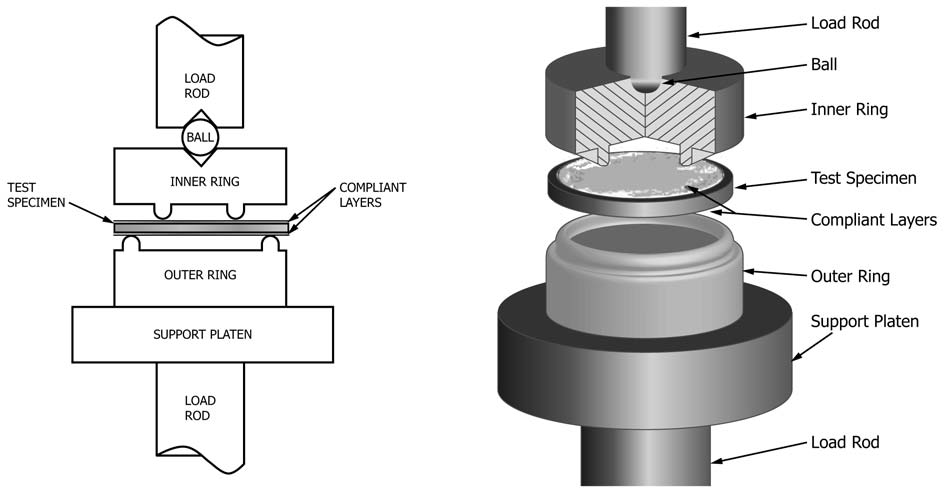
\includegraphics[width=0.7\linewidth]{./BD_3}
\caption{}
\label{fig:BD_3}
\end{figure}
\begin{figure}[!h]
\centering
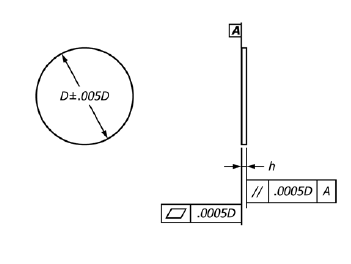
\includegraphics[width=0.7\linewidth]{./BD_2}
\caption{}
\label{fig:BD_2}
\end{figure}
\begin{figure}[!h]
\centering
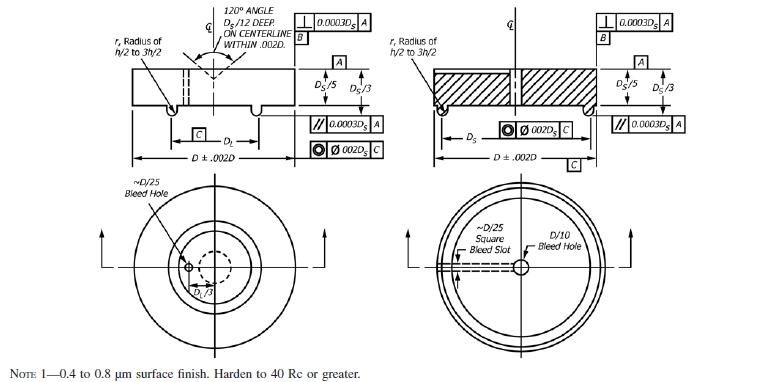
\includegraphics[width=0.7\linewidth]{./BD_1}
\caption{}
\label{fig:BD_1}
\end{figure}
\begin{figure}[!h]
\centering
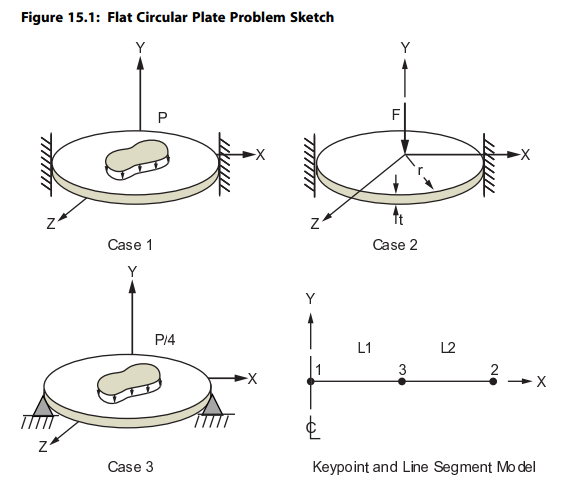
\includegraphics[width=0.7\linewidth]{./BD_4}
\caption{}
\label{fig:BD_4}
\end{figure}


\section{Closed form solution}

See Ansys Verification Problems p55

The equation for the displacement of the center of the plate is as follows:

\begin{equation}
\delta=
\frac{3F(1-\nu^2)D_L^2}{8\pi Eh^3}
\left(
\frac{D_S^2}{D_L^2}\left[1+
\frac{(1-\nu)(D_sS^2-D_L^2)}{2(1+\nu)D^2}\right]
-\left(1+\ln\frac{D_s}{D_L}\right)\right)
\end{equation}

Vitmar, F. F., and Pukh, V. P., ``Method of Determining Sheet Glass
Strength," Zavodskava Laboratoriya, Vol. 29, No. 7, 1963, pp.
863-867.


\chapter{Example 3: Thick/thin walled pressure vessel}
Abaqus verification 1.3.4
\section{Closed form solution}
The radial displacement of a thick walled pressure vessel at radius $r$ is:
\begin{equation}
u(r)=\frac{1-\nu}{E}
\frac{(r_i^2p_i-r_o^2p_o)r}{r_o^2-r_i^2}+
\frac{1+\nu}{E}
\frac{(p_i-p_o)r_i^2r_o^2}{(r_o^2-r_i^2)r}
\end{equation}

\chapter{Pressure vessel with hemispherical end-cap}
\begin{figure}[!h]
\centering
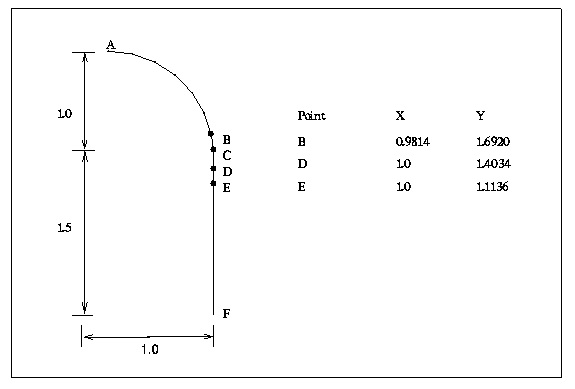
\includegraphics[width=0.7\linewidth]{./PV_1}
\caption{}
\label{fig:PV_1}
\end{figure}

\chapter{Belleville Washer}

See Ansys Verification Problems p73.
\begin{figure}[!h]
\centering
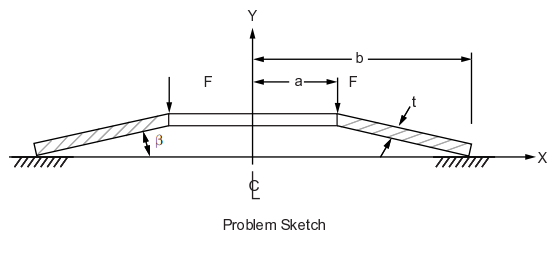
\includegraphics[width=0.7\linewidth]{./Belleville}
\caption{}
\label{fig:Belleville}
\end{figure}


\chapter{Method of manufactured solutions}

\chapter{How do we construct the elements}
we need to fix the pyfem2 element in a couple of places.
\begin{itemize}
\item Fix the B matrix so that we have the r term and shape function in the 3rd row of the B matrix. (Like we did in Homework 7)
\item Fix the integrand of the K stiffness to include the r term $B^TEBrJ_\omega$
\item Similarly fix the F term in the forcing function portion of the code.
\end{itemize}

The types of elements that we're going to focus on in this project is the reduced integration.

Secondary to those, we can optionally figure out the full integration. 

Listed out the order of attack for the elements we develop could be:
\begin{itemize}
\item Full integration (maybe easiest to implement)
\item Reduced integration (down to one gauss point)
\item Selectively reduced integration ????
\item Reduced integration with hourglass control ???
\end{itemize}

The key for our project is to get the testing framework up and running for several types of loading conditions and provide something for elements to be tested against. This testing framework is the most likely thing that Fuller will re-use in pyfem2. That's most likely what he wants.


\end{document}